\chapter{Komponenten}
\section{Webcrawler}
\subsection{Beschreibung der Technologie}
\subsubsection{Apache Storm}
StormCrawler basiert auf Apache Storm, einem Opensource Framework zur verteilten Stream-Verarbeitung.
Die Architektur von Apache Storm basiert auf den folgenden Komponenten:
\begin{itemize}
	\item Spout - Komponente zum Einlesen von Daten-Streams
	\item Bolt - Komponente zum Verarbeiten von Daten-Streams
	\item Tupel - Datensatz, welcher zwischen den Komponenten weitergegeben wird
	\item Topologie - Ein Netz bestehend aus Spouts und Bolts
\end{itemize}
Jede Komponente ist als eigene Java-Klasse definiert und beinhaltet zwingend die folgenden Methoden:
\begin{itemize}
	\item declareOutputFields() - Definition des Ausgabeschemas des Tupels
\end{itemize}
Jeder Bolt enthält zudem eine weitere Methode:
\begin{itemize}
	\item execute() - Ausführen des Tasks der Komponente
\end{itemize}
In einer Topologie werden verschiedene Spouts und Bolts miteinander verknüpft, um einen Prozess durchzuführen, wie in \cref{fig:topology} gezeigt wird.
\begin{figure}[H]	
	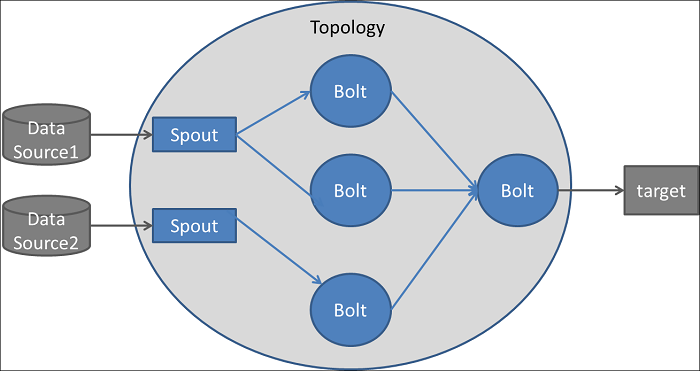
\includegraphics[width=0.8\columnwidth,keepaspectratio]{img/storm-topology.png}
	\caption{Beispieltopologie}
	\source{Quelle: https://dzone.com/articles/apache-storm-architecture}
	\label{fig:topology}
\end{figure}
Dabei hat der Spout die Aufgabe, Daten aus einer Quelle (z.B. Datei, Datenbank, Array) einzulesen und daraus ein Tupel zu bilden.
Dieses Tupel wird an die weiteren Bolts der Topologie weitergegeben und von diesen verarbeitet.
Diese Verarbeitung muss nicht seriell stattfinden, die Topologie kann auch Gabelungen beinhalten, die dementsprechend Bolts benötigen, welche entscheiden, an welchen Folge-Bolt das Tupel weitergegeben werden soll.
Zudem ist eine Webapplikation verfügbar, die eine Übersicht über die Informationen wie eine Topologieübersicht, der Status der jeweiligen Komponenten sowie Fehlermeldungen anzeigt.
\subsubsection{StormCrawler SDK}
StormCrawler ist ein Opensource Software Development Kit, welches auf Apache Storm aufbaut und in Java entwickelt wurde.
Er dient als Baukasten, um einen Webcrawler aufzubauen, der skalierbar, stabil und sehr effizient ist.
Er beinhaltet verschiedene Spouts und Bolts, die explizit zum Crawlen von Websites vorgefertigt wurden.
Zudem berücksichtigt er die Regeln des Webcrawlings, also Meta-Tags oder Robot.txt Dateien, welche deklarieren, ob eine Website gecrawlt werden darf.
Weiter ist er so eingerichtet, dass Webpages derselben Website mit einer Zeitverzögerung abfragt, damit diese nicht überlastet werden.
StromCrawler ist standardmässig so eingerichtet, dass nur Webpages desselben Hosts gecrawlt werden.
\subsubsection{Docker}
In diesem Kontext wird Docker als die Software zum Erstellen von Linux-Containern verwendet.
Mithilfe von Docker können ressourcenarme, modulare virtuelle Maschinen erstellt werden, welche auch Container genannt werden.
Diese Container können dann einfach kopiert, ersetzt oder auf einem anderen System verwendet werden \cite{DockerRetHat}.\\
Linux-Container verwenden den Linux-Kernel und seine Funktionen, einzelne Prozesse isolieren zu können.
Der Vorteil von Containern ist, dass alle Abhängigkeiten mit der ausführbaren Software in den Container gepackt werden können und somit jede Umgebung, die den gleichen Container verwendet, auch den gleichen Softwarestand besitzt.
Docker Container werden mit einem einzigen Konfigurationsfile beschrieben.
Dieses Konfigurationsfile, das sogenannte Dockerfile, definiert alle Notwendigkeiten, um den Docker Container zu realisieren.
Im Dockerfile werden Instruktionen für das Erstellen des Images definiert.
Da Dockerfiles einfache Textdateien sind, können sie, wie jeder andere Sourcecode, mit Git, SVN oder anderen Versionsverwaltungen verwaltet werden.
Aus Dockerfiles werden Docker Images erstellt.
Durch Dockerfiles können Docker Images erstellt werden, welche wiederum den dadurch definierten Container erstellen und starten.
Grundsätzlich kann das Docker Image mit einer Klasse im Objekt-Orientierten-Programmieren verglichen werden und der Docker Container wäre eine laufende Instanz der entsprechenden Klasse. 
%\footnote{\url{https://stackoverflow.com/questions/3175105/inserting-code-in-this-latex-document-with-indentation}}

\subsubsection{Docker-Compose}
Mit Docker Containern können auch Micro-Services Architekturen realisiert werden, wodurch jeder Container einen eigenen Service darstellt.
Das manuelle Starten jedes einzelnen Containers erweist sich jedoch als ineffizient, deswegen übernimmt die Software \glqq Docker-Compose\grqq{} diese Aufgabe.
Mithilfe von Docker-Compose können mehrere Docker Container verknüpft und gleichzeitig gestartet werden.
Die Abhängigkeiten zwischen den Containern wird ebenfalls mit einem Konfigurationsfile, dem Composefile, definiert.
Wahlweise können Dateiordner vom Hostsystem in einzelne Container angehängt werden, damit die Container Daten dort abspeichern oder abrufen können.
Dies ist insofern wichtig, da sobald die Container gestoppt werden, all ihre internen Daten verloren gehen.
Die Containerinhalte existieren nur so lange, wie auch die Container existieren.
Docker-Compose erstellt für alle Container in einer Gruppierung einzigartige ID-Namen, damit alle Container innerhalb der Gruppierung miteinander kommunizieren können.
\subsection{Konfiguration des StormCrawlers}
Die Grundlage der Konfiguration ist die Standardtopologie des Stromcrawlers auf Github.
\footnote{\url{https://docs.docker.com/develop/develop-images/dockerfile_best-practices/}}
Diese besteht aus den folgenden Komponenten und geht wie folgt vor:
\begin{enumerate}
	\item MemorySpout - Einlesen einer URL aus einem Array
	\item URLPartitionerBolt - Geneneriert einen eindeutigen Partition Key
	\item FetcherBolt - Ruft die Webpage ab
	\item SiteMapParserBolt - Erkennt die Sitemap-Datei und fügt weitere URLs zum MemorySpout hinzu
	\item FeedParserBolt - Extrahiert URLs aus Feeds
	\item JSoupParserBolt - Extrahiert Informationen wie Metatags oder den Text aus der Webpage
	\item SdtOutIndexer - Gibt die Informationen einer Webpage über die Konsole aus
\end{enumerate}
Ein selbst erstellter Bolt, welcher für das Schreiben des Outputs zuständig ist hat in dieser Konfiguration den StdOutIndexer ersetzt.
Dieser schreibt für jede Webpage, die erreichbar ist und gecrawlt werden darf, eine JSON Datei mit den folgenden Informationen:
\begin{itemize}
	\item \glqq date\grqq{} - Zeitpunkt, zu welchem die Webpage aufgerufen wurde
	\item \glqq text\grqq{} - Vom Webcrawler extrahierter Text, welcher die Webpage beinhaltet
	\item \glqq encoding\grqq{} - Das von der Webpage verwendete Encoding
	\item \glqq title grqq{} - Inhalt des gleichnamigen HTML-Metatags
	\item \glqq url\grqq{} - URL der Webpage
	\item \glqq content\grqq{} - Der statische HTML-Inhalt der Webpage	
\end{itemize}
Der Dateiname dieser JSON Dateien wird aus der URL der Webpage generiert. 
Sonderzeichen, die in Dateinamen nicht erlaubt sind, werden entfernt. Falls die URL länger ist, als die erlaubte Dateinamenslänge, wird diese abgeschnitten und mit einem zufälligen vierstelligen Suffix erweitert.
Zudem kommt darin eine Spracherkennung \glqq Lingua\footnote{\url{https://github.com/pemistahl/lingua}}\grqq{} zum Einsatz, welche anhand des Textes einer Webpage detektiert, ob sie mehrheitlich in deutsch geschrieben wurde.
Als deutsch detektierte Webpages werden in einen separaten Output-Ordner gespeichert, damit diese nachfolgend von Hand gelabelt werden können.
Trotzdem ist es wichtig, dass alle aufgerufenen Webpages gespeichert werden, damit im Anschluss des Crawlens eine Aussage gemacht werden kann, wie viele Einträge des Seeds effektiv gecrawlt wurden.

\section{Klassifizierung}
\subsection{Verwendete Technologien}
\subsubsection{Luigi}
Luigi ist ein Pipelining-Tool, welches von Spotify entwickelt und später als Open-Source Projekt veröffentlicht worden ist.\footnote{\url{https://github.com/spotify/luigi}}
Pipelining dient dazu, mehrere Tasks miteinander zu verknüpfen, das Ausführen zu Automatisieren und somit eine grössere Aufgabe zu verrichten.
Pipelining wird meist im Kontext von Big Data oder Machine-Learning angewendet, wo sich viele einzelne Tasks mit grossen Datenmenge beschäftigen.
Luigi wird selbst von Spotify in der produktiven Umgebung verwendet und bietet unter anderem folgende Features:
\begin{itemize}
	\item Einzelne Tasks idempotent ausführen
	\item Teilschritte oder gesamte Pipeline kann über Konsolenausgabe oder Webinterface überwacht werden
	\item Fehlerfälle können protokolliert werden und dementsprechend reagiert werden
	\item Abhängigkeiten von Tasks werden selbstständig von Luigi gelöst
	\item Luigi ist komplett in Python aufgebaut und kann auch mit Python konfiguriert werden
\end{itemize}
Die einzelnen Tasks werden mit Python-Klassen realisiert.
Luigi ist so aufgebaut, dass jeder Task ein Input-File liest, von dem die Ausgabe des vorherigen Tasks eingelesen wird und ein Output-File schreibt, welches als Input-File des anschliessenden Tasks benutzt wird.
Dadurch kann Luigi die Zustände der einzelnen Tasks überwachen und bei einem Fehlerfall die Pipeline dort wieder starten, wo sie sich aufgehängt hat.
Damit Luigi die Abhängigkeiten und das Überwachen bewerkstelligen kann, benötigt jede Klasse in der Pipeline folgende drei Funktionen:
\begin{itemize}
	\item Funktion requires(), Angabe auf welche Tasks Abhängigkeiten bestehen
	\item Funktion run(), Bereich, wo die eigentliche Logik des Tasks ist
	\item Funktion output(), wohin die Ausgabe geschrieben wird
\end{itemize}
In dieser Arbeit wurde Luigi verwendet, um die Klassifizierung zu verknüpfen.

Es wurden zwei verschiedene Arten von Pipelines erstellt.
Die Entwicklungspipeline diente zur Entwicklung der Regeln/Machine-Learning-Modelle für die Klassifizierung.
Die Klassifizierung beinhaltet das Lesen der gecrawlten Daten, das Preprocessing, das Klassifizieren und das Evaluieren der Klassifizierung.
Die daraus folgende Pipeline beinhaltet folgende Tasks:
\begin{itemize}
	\item Importer, import die gecrawlten Websites und speichert sie in einer CSV-Datei
	\item Preprocessor, wendet übliche Preprocessing-Schritte an den Daten an
	\item RuleBasedClassifier, regelbasierte Klassifizierung der Daten 
	\item MLClassifier, Klassifizierung der Daten mittels Machine-Learning
	\item Evaluator, Auswertung der Klassifizierung von Daten (Nur im Entwicklunsmodus)
\end{itemize}
\subsubsection{Scikit Learn}
Scikit Learn ist eine freie Programmierbibliothek für Python, mit welcher man effizient Projekte für Data-Mining, Datenvisualisierung und Machine-Learning erarbeiten kann.
Scikit Learn ist unter BSD lizenziert und für den kommerziellen Nutzen frei verfügbar.
Sie ist eine der bekanntesten Standardbibliotheken für Machine-Learning, wird unter anderem von grossen Namen wie Google finanziell unterstützt und besitzt eine rege Contribution-Community auf Github\footnote{\url{https://github.com/scikit-learn/scikit-learn}}.\\
Scikit Learns Stärken liegen in den Machine-Learning Bereichen \glqq Supervised Learning\grqq{} und \glqq Unsupervised Learning\grqq{}.
Die API von Scikit Learn bietet eine Vielzahl von Algorithmen für Klassifizierung, Regression, Clustering, Dimensionsreduktion, Modelselektion und Preprocessing an und deckt somit die ganze Machine-Learning Pipeline ab.\footnote{\url{https://scikit-learn.org/stable/}}
Scikit Learn bietet für fast jeden Algorithmus oder Technik in der API eine Beispielimplementation an, welche für Fast-Prototyping  als Fundament übernommen werden kann.
\subsection{Preprocessing}\label{preprocessing}
Das Preprocessing wurde entwickelt, um den Inhalt des Dokuments auf eine standardisierte Form zu bringen.
Die folgenden Methoden können sowohl auf den Text eines Dokuments sowie auch auf den Titel angewendet werden.
Diese werden sequenziell in der unten aufgeführten Reihenfolge angewandt und können mittels Konfiguration sowohl für den Text als auch Titel eines Dokuments ein- oder ausgeschaltet werden.
\subsubsection{Gross-/Kleinschreibung}
Alle Buchstaben, welche grossgeschrieben sind, werden durch die entsprechenden Kleinbuchstaben ersetzt.
\subsubsection{Umlaute ersetzen}
Umlaute werden durch ihre verwandten Selbstlaute ersetzt, genauer:
\begin{itemize}
	\item ä $\rightarrow$ a
	\item ö $\rightarrow$ o
	\item ü $\rightarrow$ u
\end{itemize} 
\subsubsection{Preisdetektor}
Da Menüs häufig in Verbindung mit Preisen vorkommen und in weiteren Preprocessing-Schritten Zahlen und Sonderzeichen entfernt werden, ist es von Vorteil, diese Informationen nicht zu verlieren.
Daher erkennt diese Methode verschiedene Varianten von Preisen mittels Regulären Ausdrücken (Regex, Regular Expression) und ersetzt diese mit einem Schlüsselwort.
% Varianten genauer ausführen
Die folgenden Varianten von Preisen wird erkannt:
\begin{itemize}
	\item preisangabe + chf/fr/sfr
	\item preisangabe
	\item chf/fr/sfr + preisangabe
\end{itemize} 
Zudem wird unterschieden, wie viele Stellen der Preis hat.
Die nun aufgeführte Liste zeigt die verschiedenen Schlüsselwörter:
\begin{itemize}
	\item Einstellig $\rightarrow$ onedigitprice
	\item Zweistellig $\rightarrow$ twodigitprice
	\item Dreistellig $\rightarrow$ threedigitprice
\end{itemize} 
Um Zeitangaben nicht als Preise zu erkennen, werden bei Preisangaben ohne Währungsangabe nur Beträge mit Rappenbeträgen, welche 60 oder höher sind, erkannt.
\subsubsection{Sonderzeichen entfernen}
Alle Sonderzeichen, die nicht in der folgenden Auflistung vorkommen, werden durch einen Leerschlag ersetzt:
%Eventuell noch anpassen, da Grossbuchstaben nicht mehr relevant sind (EVTL. é usw auch noch ersetzen?)
\begin{itemize}
	\item éàèÉÀÈäöüÄÖÜa-zA-Z
\end{itemize} 
\subsubsection{Einzelne Zeichen entfernen}
Jedes einzelne Zeichen, also solche, die sowohl vorne als auch hinten an einen Leerschlag angrenzen, werden entfernt.
\subsubsection{Multiple Leerschläge entfernen}
Da durch die vorhergehenden Schritte oft multiple Leerschläge anfallen, werden diese auf einen Leerschlag reduziert.
\subsubsection{Stammformreduktion}
Dieses Verfahren führt verschiedene morphologische Varianten eines Wortes auf ihren gemeinsamen Stamm zurück.
Dafür wird der Stemmer \glqq Cistem\footnote{\url{https://github.com/LeonieWeissweiler/CISTEM}}\grqq{} verwendet, da für die deutsche Sprache nur wenig Alternativen vorhanden sind. 
\subsubsection{Getränkedetektor}
% Referenz Cistem
Eine Liste mit Einträgen diverser Getränke bildet die Grundlage dieser Methode.
Wenn im Text ein Getränk dieser Liste vorhanden ist, wird es durch das Schlüsselwort \glqq beverageentity\grqq{} ersetzt.
Damit soll erreicht werden, dass ein einheitliches Merkmal geschaffen wird.
\subsubsection{Stoppwörter entfernen}
Bei Stoppwörter handelt es sich um Wörter, welche keine Relevanz für den Inhalt eines Texts haben, aber oft vorkommen.
Eine Stoppwortliste führt 1720 solcher Wörter in deutsch auf. Sie ist aus mehreren Quellen zusammengesetzt worden.
% Quellen Stoppwortliste aufführen?
Wenn eines dieser Wörter im Text vorkommt, wird es entfernt.
\subsection{Regelbasierte Klassifizierung}
Verschiedene Algorithmen kommen beim regelbasierten Klassifizieren zum Einsatz, welche nun genauer erläutert werden.
\subsubsection{Menü im Titel}
Dieser simple Algorithmus kontrolliert, ob das Wort \glqq menu\grqq{} im Metatag \glqq Title\grqq{} vorkommt.
Falls ja, wird das Dokument als Menüseite klassiert.
\subsubsection{Preisdetektor}
Dieser Algorithmus funktioniert dank der Preprocessing-Methode, welche den Preis erkennt und mit einem Schlüsselwort ersetzt.
Sofern dieses Schlüsselwort im Text vorhanden ist, wird das Dokument als Menüseite klassifiziert. Dies unter der Annahme, dass Menüpreise oft zweistellig sind, im Gegensatz zu Getränkepreisen welche häufig einstellig sind und Hotelpreisen, die meist dreistellig sind.
Die Anzahl vorhandener Preise kann über die Konfiguration angegeben werden.
\subsubsection{Kombination aus Menü im Titel und Preisdetektor}
Diese Kombination führt eine sequenzielle Klassifikation aus.
Im ersten Schritt wird der Mechanismus des Algorithmus \glqq Menü im Titel\grqq{} verwendet.
Falls durch diesen keine positive Klassifikation zustande kommt, wird durch den Preisdetektor nochmals neu klassifiziert.
\subsubsection{Listing}
Dieser Algorithmus basiert sowohl auf dem Black- als auch auf dem Whitelisting Ansatz.
Dazu wird eine Blacklist und eine Whitelist verwendet, die von Hand erstellt wurden und Einträge enthalten, welche für die jeweiligen Kategorien typisch sind.
Falls ein Wort einer Liste im Text einer Webpage vorkommt, wird ein entsprechender Zähler hochgezählt.
Zum Schluss findet eine sequenzielle Klassifizierung statt, das heisst: 
Wenn der Zähler der Blacklist einen konfigurierbaren Schwellwert überschreitet, wird die Webpage als negativ klassifiziert. 
Wenn der Zähler der Whitelist einen konfigurierbaren Schwellwert überschreitet, wird die Webpage als Menüseite klassifiziert.
Falls keiner der beiden Zähler den Schwellwert überschreitet, wird die Webpage ebenfalls als negativ klassifiziert. 
\subsubsection{Bag of Words}
Dieser Algorithmus basiert auf dem statistischen Ansatz namens \glqq Bag of Words\grqq{}.
Dafür wird der komplette Datensatz in einen Trainings- und Testsatz in einem konfigurierbaren Verhältnis aufgeteilt.
Bag of Words zählt für jedes Dokument der Trainingsdaten, wie oft ein Wort darin vorkommt.
In dieser Anwendung wird jedoch nur erkannt, ob ein Wort vorkommt, oder nicht, die Anzahl spielt keine Rolle.
Anhand dieser Wörter wird eine dynamische Black- und Whitelist erstellt, Wörter die in beiden Listen vorkommen, werden entfernt.
Anhand dieser Listen wird der Testdatensatz klassifiziert.
Die Anzahl der Wörter dieser Listen ist konfigurierbar.
Die Klassifikation findet mittels einem Zähler statt.
Für jedes Wort eines Dokuments, welches in der Liste der positiven Beispielen vorkommt, wird der Zähler hochgezählt, für jedes Wort aus der Liste der negativen Beispielen wird er heruntergezählt.
Für die Klassifizierung wird der Zähler mit einem konfigurierbaren Schwellwert verglichen, Falls der Zähler grösser ist als der Schwellwert, wird das Dokument als positiv klassifiziert, ansonsten negativ.
Um die Ergebnisse anhand der Testdaten evaluieren zu können, sind diese Listen zudem statisch implementiert worden.
Ob diese dynamisch erzeugt werden oder die statisch implementierten Listen verwendet werden sollen, kann mittels Konfigurationsoption gewählt werden.
\subsection{Feature-relevante Methoden für Machine-Learning}
\subsubsection{Bag of Words}
Der statistische Ansatz namens \glqq Bag of Words\grqq{} wandelt einen Text in eine Anhäufung von Wörtern um.
Danach wird für jedes Wort die Häufigkeit des Vorkommens in dieser Anhäufung gezählt und hinterlegt.
Bag of Words erstellt im Grunde ein Histogramm aller Wörter eines Textes.
Ebenfalls kann die boolsche Häufigkeit (Term vorhanden/nicht vorhanden) verwendet werden, damit man nur ein Set von allen im Text vorkommenden Wörtern erhält.
\subsubsection{TF-IDF}
TF-IDF (TermFrequency-InverseDocumentFrequency) ist eine Methodik zur Bestimmung der Relevanz eines Terms in einer Sammlung von Dokumenten (Dokumentkorpus).\\
TF-IDF wird aus den zwei folgenden Metriken zusammengesetzt.
\begin{itemize}
	\item TF
	\begin{itemize}
		\item Termfrequenz berechnet das Vorkommnis eines Termes in einem Dokument. Anschliessend wird das Vorkommnis mit der gesamten Anzahl von Termen im Dokument dividert. Dies erreicht eine Normalisierung der Termfrequenz, da bei langen Texten der Term potentiell öfters vorkommen kann.\\
		TF verfolgt einen ähnlichen Ansatz wie Bag of Words.
	\end{itemize}
	\item IDF
	\begin{itemize}
		\item TF ermittelt nur die Häufigkeit der Terme. Terme wie \glqq die\grqq{} oder ähnliche kommen oft vor, sind aber nicht relevant.\\
		IDF ermittelt nun die Relevanz der Terme indem berechnet wird, wie viele Dokumente den Term T in sich enthalten. Die gesamte Anzahl an Dokumenten wird durch die ermittelte Anzahl von Dokumenten mit Term T dividiert und mit dem natürlichen Logarithmus logarithmiert.\\
		Somit ist ein Term, welcher in vielen Dokumenten vorkommt, weniger relevant als ein rarer Term.
	\end{itemize}
	\item TF-IDF
	\begin{itemize}
		\item TF-IDF ist nun die Multiplikation von TF und IDF.
	\end{itemize}
\end{itemize}
TF-IDF stammt aus der Disziplin \glqq Information Retrieval\grqq{} und findet dank der Gewichtung von Wörtern im Machine-Learning Bereich hohen Anklang.\footnote{\url{http://www.tfidf.com/}}
\subsubsection{Latent Semantic Analysis}
LSA basiert auf der Scikit-Implementation\footnote{\url{https://scikit-learn.org/stable/modules/decomposition.html}} von \glqq Single Value Decomposition SVD\grqq{}oder auf deutsch \glqq Singulärwertzerlegung\grqq{}.
SVD zerlegt die Termdokumentmatrizen, welche von den Scikit-Learn Bag of Words oder TF-IDF Algorithmen erstellt werden, in ihre K wichtigsten Werte. Wobei K frei gewählt werden kann, jedoch kleiner als die maximale Anzahl von Features aus Bag of Words oder TF-IDF sein muss.
Wenn SVD explizit auf Termdokumentmatrizen angewendet wird, wird der Vorgang \glqq Latent Semantic Analysis\grqq{} oder auch \glqq Latent Semantic Indexing\grqq{} genannt.
Dies hat der Grund, da die Matrizen in semantische Matrizen kleinerer Dimension umgewandelt werden.\\
Ein Vorteil von LSA ist, es kann Synonyme, mehrere Wörter mit gleicher Bedeutung, erkennen und somit die Termdokumentmatrizen dementsprechend reduzieren, jedoch ohne grosse Verluste in der Aussagekraft zu erleiden.
\subsection{Machine Learning Algorithmen}
\subsubsection{Übersicht}
Wegen des "No free lunch"-Theorems wurden 14 Algorithmen stetig trainiert und validiert.
Nun erfolgt eine Auflistung aller Algorithmen, die verwendet wurden.
\begin{itemize}
	\item Lineare Modelle
	\begin{itemize}
		\item Ridge Classifier
		\item Perceptron
		\item PassiveAgressiveClassifier
		\item SGDClassifier (Stochastic Gradient Descent)
	\end{itemize}
	\item Naive Bayes Modelle
	\begin{itemize}
		\item Bernoulli-Naive-Bayes
		\item Complement-Naive-Bayes
		\item Multinomial-Naive-Bayes
		\item Gaussian-Naive-Bayes
	\end{itemize}
	\item Tree Modelle
	\begin{itemize}
		\item DecisionTreeClassifier
	\end{itemize}
	\item Ensemble Modelle
	\begin{itemize}
		\item RandomForestClassifier
		\item AdaBoostClassifier
	\end{itemize}
	\item Nearest Neighbor Modelle
	\begin{itemize}
		\item KNeighborClassifier
		\item Nearest Centroid
	\end{itemize}
	\item Support Vector Machines Modelle
	\begin{itemize}
		\item LinearSVC (Support Vector Classification)
	\end{itemize}
\end{itemize}
Jedoch nur die Algorithmen, welche nach der vollständigen Ausführung aller Optimierungsschritte die höchsten F1-Scores oder Precisions erzielt haben, werden weiter unten näher umschrieben.
Im Anhang können alle Klassifizierer mit ihren entsprechenden Scores eingesehen werden.
\subsubsection{SGDClassifier}
SGDClassifier gehört zur Familie der lineare Modelle.\footnote{\url{https://scikit-learn.org/stable/modules/generated/sklearn.linear_model.SGDClassifier.html}}\\
Lineare Modelle sind in der Annahme, dass ein linearer Zusammenhang zwischen Eingangsvariabeln und Ausgangsvariabeln besteht.
Lineare Modelle versuchen Parameter zu einer linearen Gleichung zu finden, welche die Trainingsdatenpunkte optimal abdeckt.
Das optimale Abdecken wird mit einer Loss-Funktion ermittelt.
Die Loss-Funktion berechnet den Unterschied zwischen vorhergesagtem Wert zu tatsächlichem Wert des Trainingsdatenpunktes.
Lineare Modelle verwenden Optimierungsverfahren, welche iterativ Parameter verändern, um die Werte der Loss-Funktion zu minimieren und somit die bestmögliche Parameterzusammensetzung zu ermitteln.\\
Der \glqq Stochastic-Gradient-Descent-Classifier\grqq{} verwendet als Optimierungsvefahren das \glqq Stochastic Gradient Descent\grqq{} Verfahren\footnote{\url{https://scikit-learn.org/stable/modules/sgd.html}}.
Bei diesem Verfahren kommt der mathematische Gradient zum Einsatz.
Der Gradient zeigt bei Anpassungen der Parameter, immer in die Richtung mit der grössten Änderung des Outputs.
Der Output wäre in diesem Falle die Aufzeichnung des Loss-Funktion.\\
Der stochastische/probabilistische Anteil dieses Verfahrens bedeutet, dass bei der Optimierung jeweils nur ein Parameter zufällig ausgesucht und angepasst wird und seine Auswirkung anschliessend ermittelt wird.
Dies hat den Vorteil, dass die Trainingszeit optimiert werden kann und zugleich gute Werte erzielt werden können.\\
In der Abbildung \cref{fig:sgd} wird der Verlauf der Loss-Funktion aufgezeigt und wie der Gradient zu interpretieren ist.
\begin{figure}[H]	
	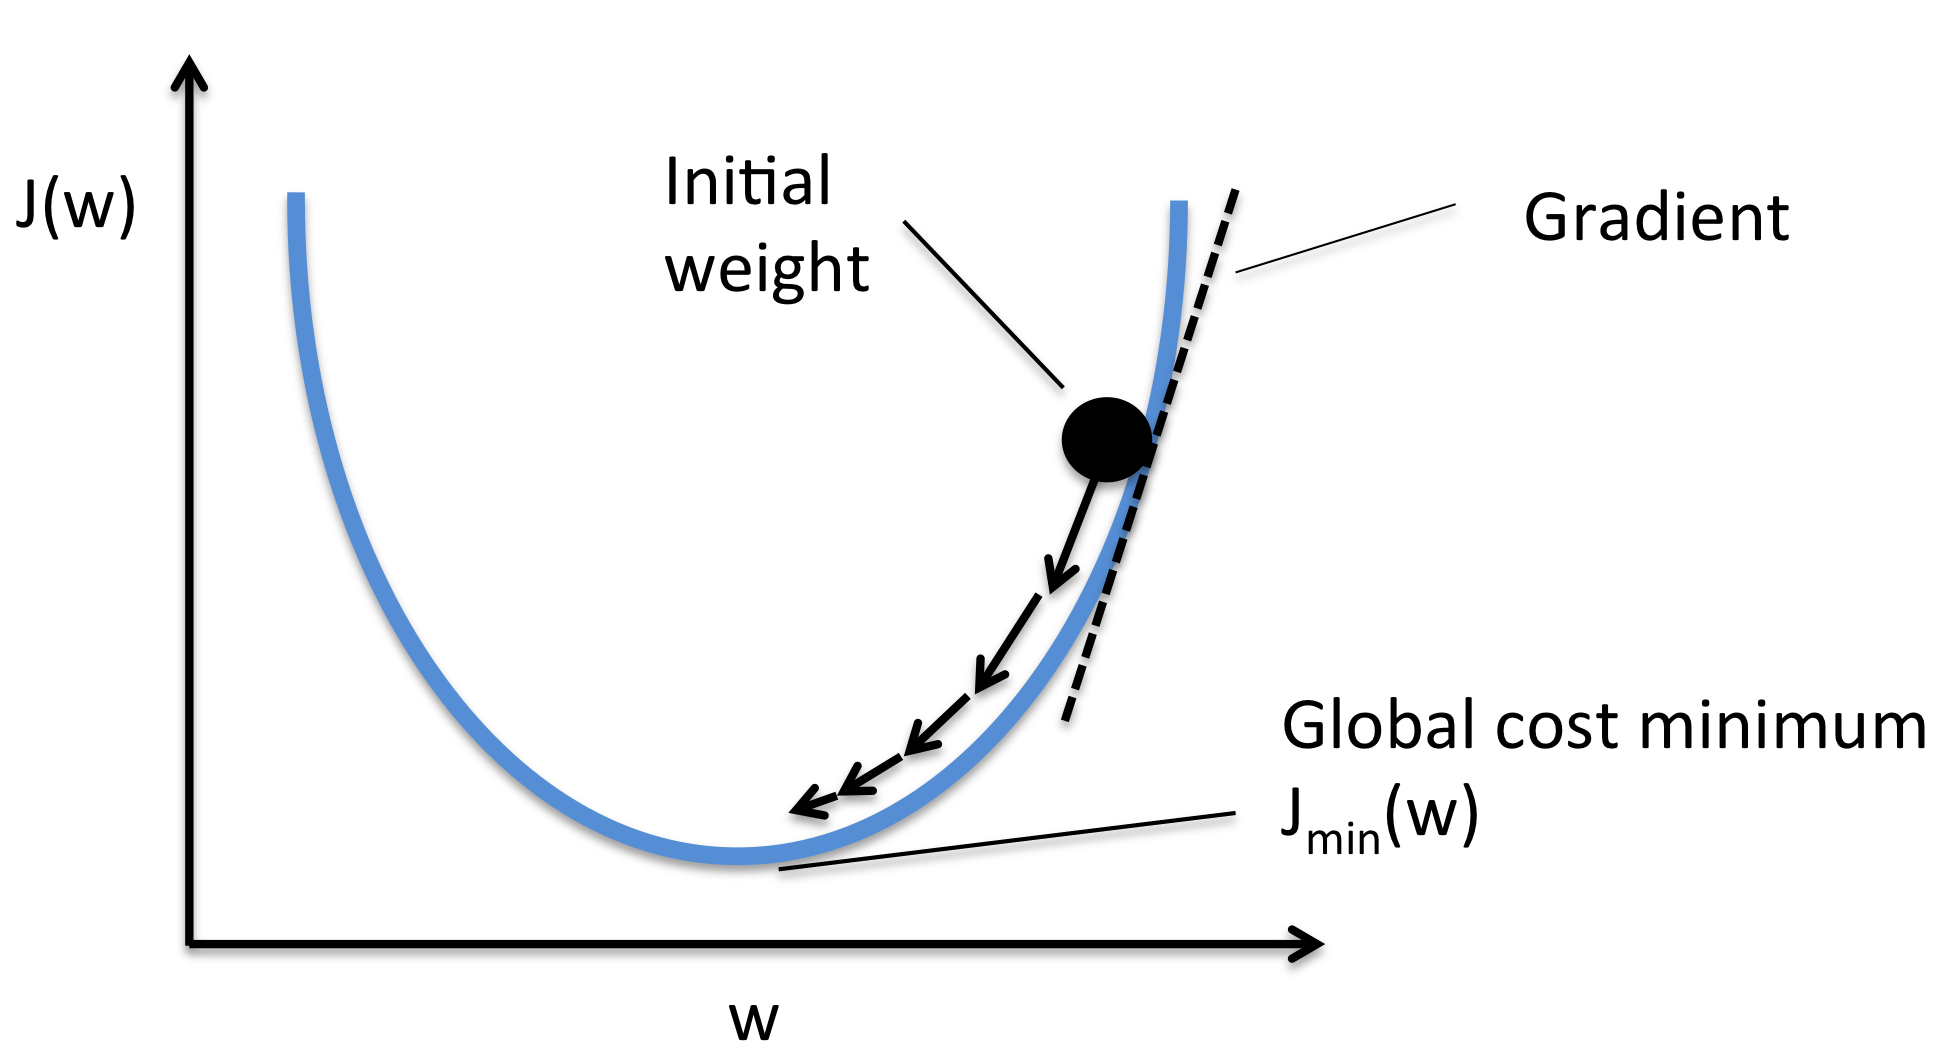
\includegraphics[width=1\columnwidth,keepaspectratio]{img/sgd.png}
	\caption{Visualisierung des Gradienten und der Loss-Funktion (J(w) = Loss; w = Parameteränderung)}
	\label{fig:sgd}
\end{figure}
\subsubsection{Perceptron}
Der Perceptron-Algorithmus basiert auf dem SGDClassifier.\footnote{\url{https://scikit-learn.org/stable/modules/generated/sklearn.linear_model.Perceptron.html}}
Hinter der Perceptron-Implementierung steckt lediglich ein SGDClassifier mit spezieller Konfiguration.\\
Die Perceptron-Implementierung benutzt in der Konfiguration die Loss-Funktion \glqq perceptron\grqq{}, keine Strafe bei falscher Klassifizierung und eine konstante Lernrate.
\subsubsection{AdaBoostClassifier}
AdaBoost gehört zu der Familie der Ensemble-Learner.\footnote{\url{https://scikit-learn.org/stable/modules/generated/sklearn.ensemble.AdaBoostClassifier.html}}
Ensemble-Learning ist ein Zusammenschluss von mehreren unterschiedlichen Klassifizieren, welche mit einem Voting-Verfahren eine schlussendliche Klassifizierung durchführen.
Ensemble-Learning verfolgt die Annahme, dass mehrere Algorithmen im Plenum eine bessere Aussage abliefern können, als einen Algorithmus alleine.
Bei vielen Ensemble-Verfahren werden alle Klassifizierer parallel trainiert und geben ihr Votum gleichzeitig ab.\\
Adaboost verwendet jedoch die Methode des \glqq Boosting\grqq{}, welche Ähnlichkeit mit der Theorie der genetischen Algorithmen hat.\footnote{\url{https://scikit-learn.org/stable/modules/ensemble.html}}
Bei Adaboost wird ein Algorithmus trainiert, validiert und als Ursprung verwendet. Alle zusätzlichen Algorithmen, welche das finale Voting durchführen, werden vom Ursprungsalgorithmus abgeleitet.
Es werden jedoch bei den Abkömmlingen die internen Parameter schrittweise verbessert und versucht die Fehler des \glqq Vater-Algorithmus\grqq{} zu vermeiden.
AdaBoost kann verbessert werden, indem die Anzahl von Vererbungsschritten angepasst wird.
\subsubsection{RandomForestClassifier}
RandomForest gehört ebenfalls zur Familie der Ensemble-Learner.\footnote{\url{https://scikit-learn.org/stable/modules/generated/sklearn.ensemble.RandomForestClassifier.html}}
RandomForest, wie der Name schon sagt, ist eine Zusammensetzung von einer Vielzahl von unterschiedlichen DecisionTrees.\\
DecisionTree ist ebenfalls ein Algorithmus, der für die Klassifizierung verwendet werden kann.
Der DecisionTree-Algorithmus baut schrittweise eine Baumstruktur von Entscheidungszweige auf, um eine Klassifizierungsaufgabe zu meistern. 
DecisionTrees können verbessert werden, indem die Tiefe der Äste oder die Anzahl der Äste angepasst werden kann.
Bei stetiger Erhöhung der Tiefe oder der Anzahl der Äste, steigt auch die Zeitkomplexität der DecisionTrees.\\
RandomForest verwendet nun eine Vielzahl von DecisionTrees, die alle unterschiedliche Tiefen oder Anzahl Äste besitzen.
Dadurch können Entscheidungsausreisser aufgefangen und durch den Mehrheitsentscheid gedämpft werden.\\
RandomForests können oft eine sehr hohen Score bei der Precision erzielen.
\subsection{Klassifizierung mittels Machine-Learning}
\subsubsection{Konfiguration}
\subsubsection{}
\subsection{Evaluierung}
Da es sich in diesem Experiment um eine binäre Klassifizierung handelt, werden Metriken wie F1-Score, Precision und Recall verwendet.
Dazu müssen zuerst die folgenden Klassifizierungskategorien erläutert werden:
\begin{itemize}
	\item Richtig Positiv: Die Webpage wurde als Menüseite klassifiziert und ist eine Menüseite
	\item Falsch Positiv: Die Webpage wurde als Menüseite klassifiziert, ist aber keine Menüseite
	\item Falsch Negativ: Die Webpage wurde nicht als Menüseite klassifiziert, ist aber eine Menüseite
	\item Richtig Negativ: Die Webpage wurde nicht als Menüseite klassifiziert und ist keine Menüseite
\end{itemize}
Jede klassifizierte Webpage lässt sich in eine dieser Kategorie einordnen.
Anhand dieser Kategorien lässt sich für den gesamten Datensatz die oben genannten Metriken berechnen:\\
\[Precision=\frac{\text{Richtig Positiv}}{\text{Richtig Positiv} + \text{Falsch Positiv}}\]\\
Die Precision definiert das Verhältnis der korrekt positiv klassifizierten Menüseiten zu allen durch den Algorithmus als positiv klassifizierten Menüseiten.\\
\[Recall=\frac{\text{Richtig Positiv}}{\text{Richtig Positiv} + \text{Falsch Negativ}}\]\\
Der Recall definiert das Verhältnis der korrekt positiv klassifizierten Proben zu allen tatsächlichen Menüseiten.\\
\[F_{1}=2*\frac{\text{Precision} \times \text{Recall}}{\text{Precision} + \text{Recall}}\]\\
Anhand des F1-Scores wird die Genauigkeit der Klassifizierung gemessen.
Für jede Methode und jede Konfiguration der Klassifizierung werden diese Scores berechnet, um eine Aussage machen zu können, wie gut sie sind.
\section{Webapplikation}
\subsection{Beschreibung der Technologie}
\subsection{Beschreibung der Architektur}
\subsection{Search Engine}
\subsubsection{Beschreibung der Technologie}
\subsubsection{Konfiguration}
